\Chapter{Tesztelés és Eredmények}

A program funkciói a fejlesztés során folyamatosan tesztelésre kerültek, alapvetően manuálisan. Az algoritmus, illetve a szemantikus verziózás tesztelése végül a statisztikai vizsgálat során automatikusan is megtörtént, bár nem ez volt annak a résznek a célja.

Ebben a szekcióban a program felhasználása, illetve a használatával szerzett eredmények elemzése kerül ismertetésre.

\Section{Az elkészült program használata}

A kész szoftver használata az egyszerű és átlátható UI miatt kényelmes, először az egy csomagot vizsgáló mód kerül bemutatásra (\ref{fig:examiner} ábra), majd a több csomag statisztikai vizsgálatáért felelős mód (\ref{fig:statistics} ábra).

\begin{figure}[!h]
	\centering
	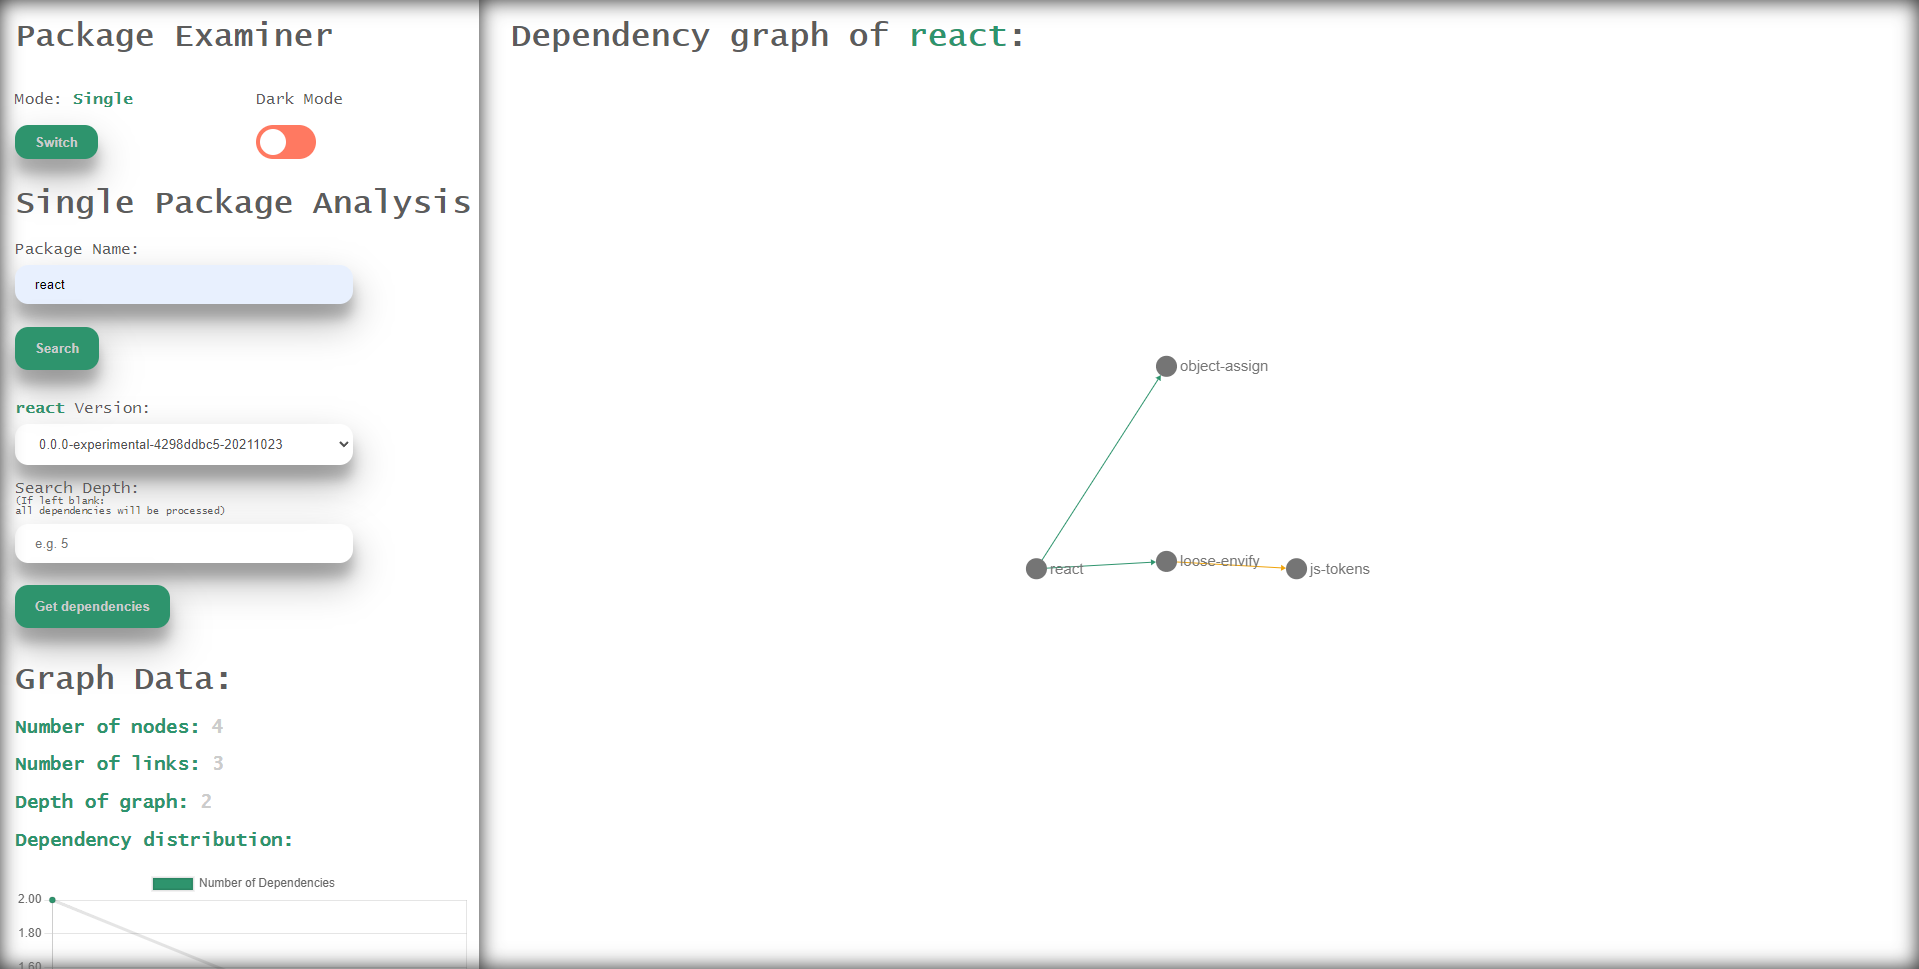
\includegraphics[scale=0.2]{images/examiner.png}
	\caption{Egy csomagos mód}
	\label{fig:examiner}
\end{figure}

\begin{itemize}
	\item Első lépésként meg kell adni a csomag nevét és keresni a (Search) gombbal.
	\item Helyes csomagnév esetén feltöltődik a verziók listája, innen tetszőlegesen kell választani egyet. Opcionálisan megadható a keresés mélysége.
	\item Végül a "Get dependencies" gomb megnyomásával lehet elindítani a folyamatot.
	\item Az elkészült ábra görgővel és egérgomb lenyomva tartásával interaktívan mozgatható, nagyítható. A Sidebar pedig lefelé görgethető a gráfelemzés információinak megtekintéséhez.
\end{itemize}

\pagebreak

A két mód közötti váltást a (Switch) gomb segítségével lehet megtenni.

\begin{figure}[!h]
	\centering
	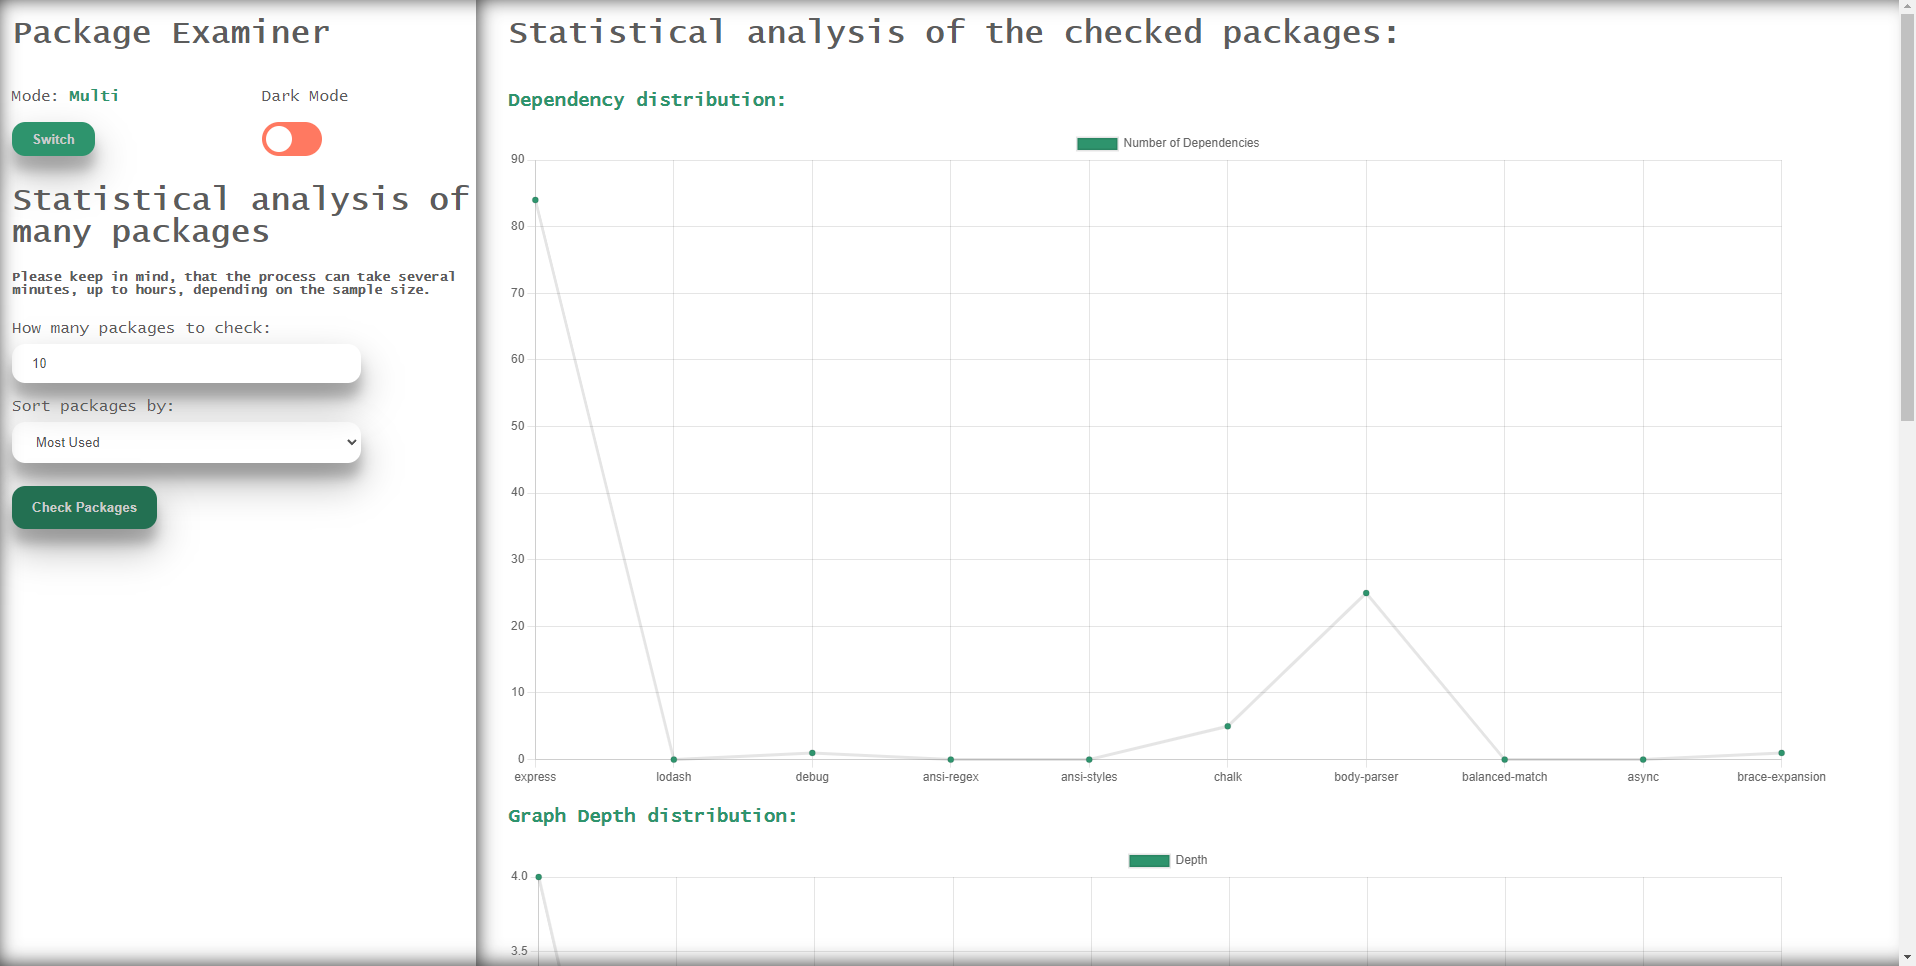
\includegraphics[scale=0.2]{images/statistics.png}
	\caption{Több csomagos mód}
	\label{fig:statistics}
\end{figure}

\begin{itemize}
	\item A több csomagos módban először a vizsgált csomagok mennyiségét szükséges megadni.
	\item A lefelé gördülő listából pedig a sorrendbe állítási elvet kell kiválasztani, alapértelmezett a leggyakrabban használt csomagok elve.
	\item A folyamatot a "Check Packages" gombra kattintással lehet elindítani.
\end{itemize}

\Section{A kapott eredmények bemutatása}

A korábban tárgyalt mérete és csomagmennyisége miatt az npm Registry egészét túl hosszas és költségigényes lenne elemezni, így az első ezer leggyakrabban használt csomagról, mint "reprezentatívan leszűkített Registryről" készült statisztikai elemzés. A vizsgálat előtt a program a csomagokat a függőségek száma szerint csökkenő sorrendbe állította, majd elvégezte a szükséges számításokat és az eredményeket a következő hisztogramokon ábrázolta:

\begin{figure}[!h]
	\centering
	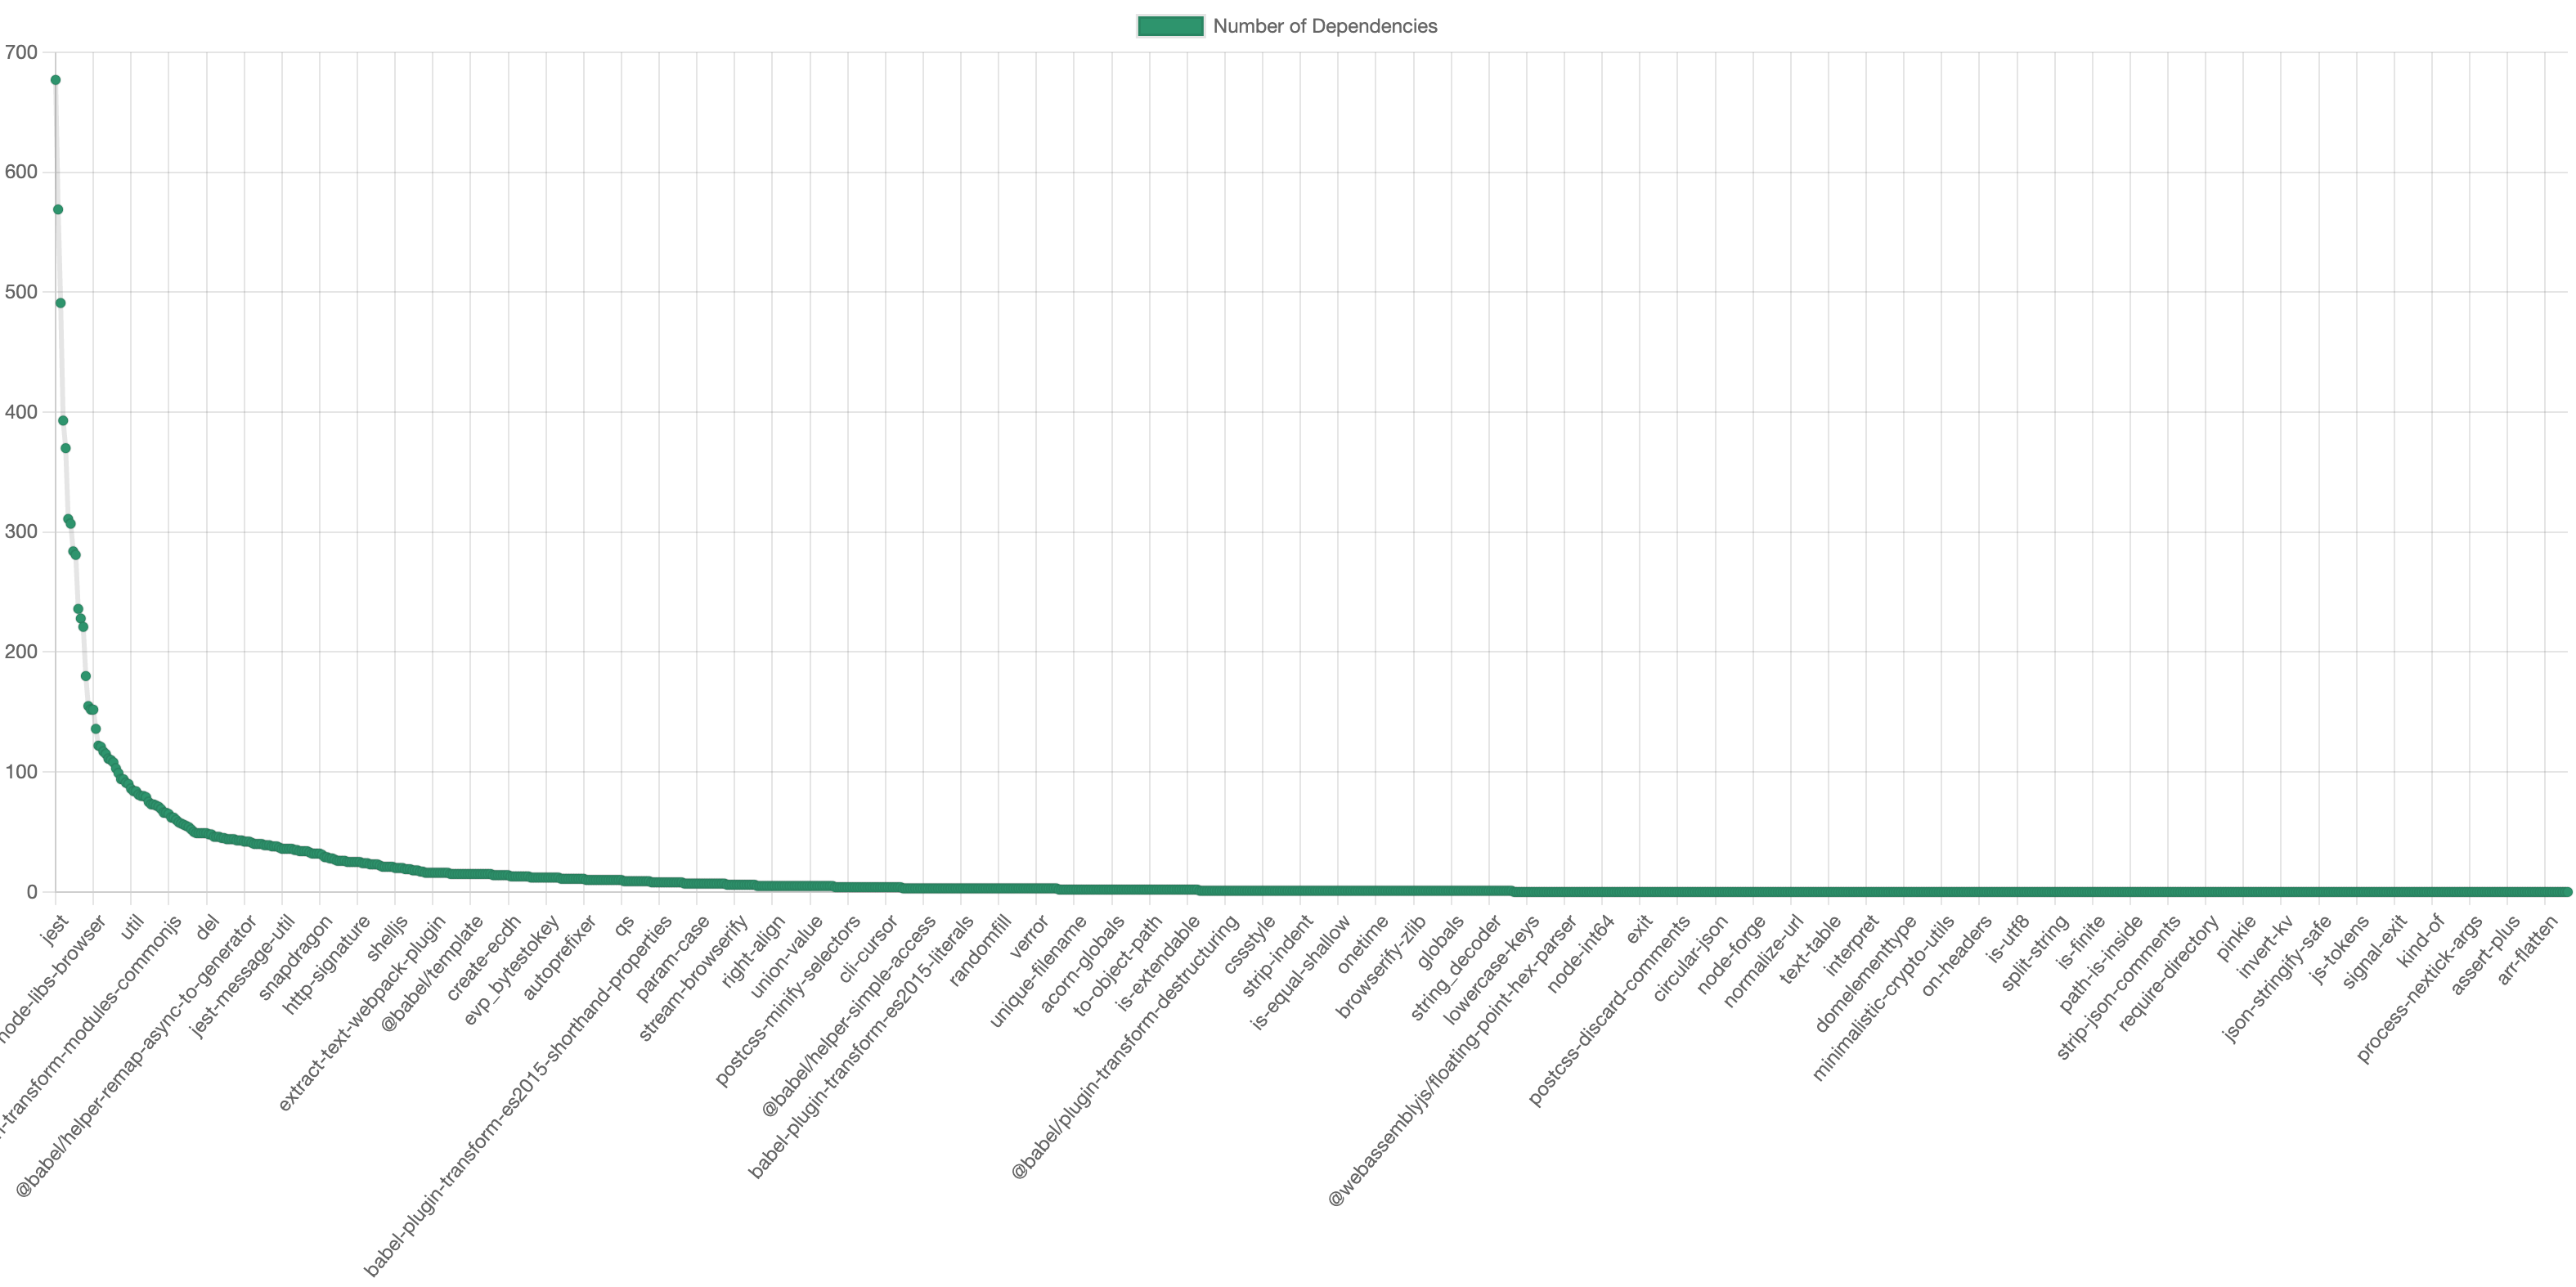
\includegraphics[scale=0.12]{images/depdist.png}
	\caption{Csomagonkénti függőségek száma}
	\label{fig:depdist}
\end{figure}  

\begin{figure}[!h]
	\centering
	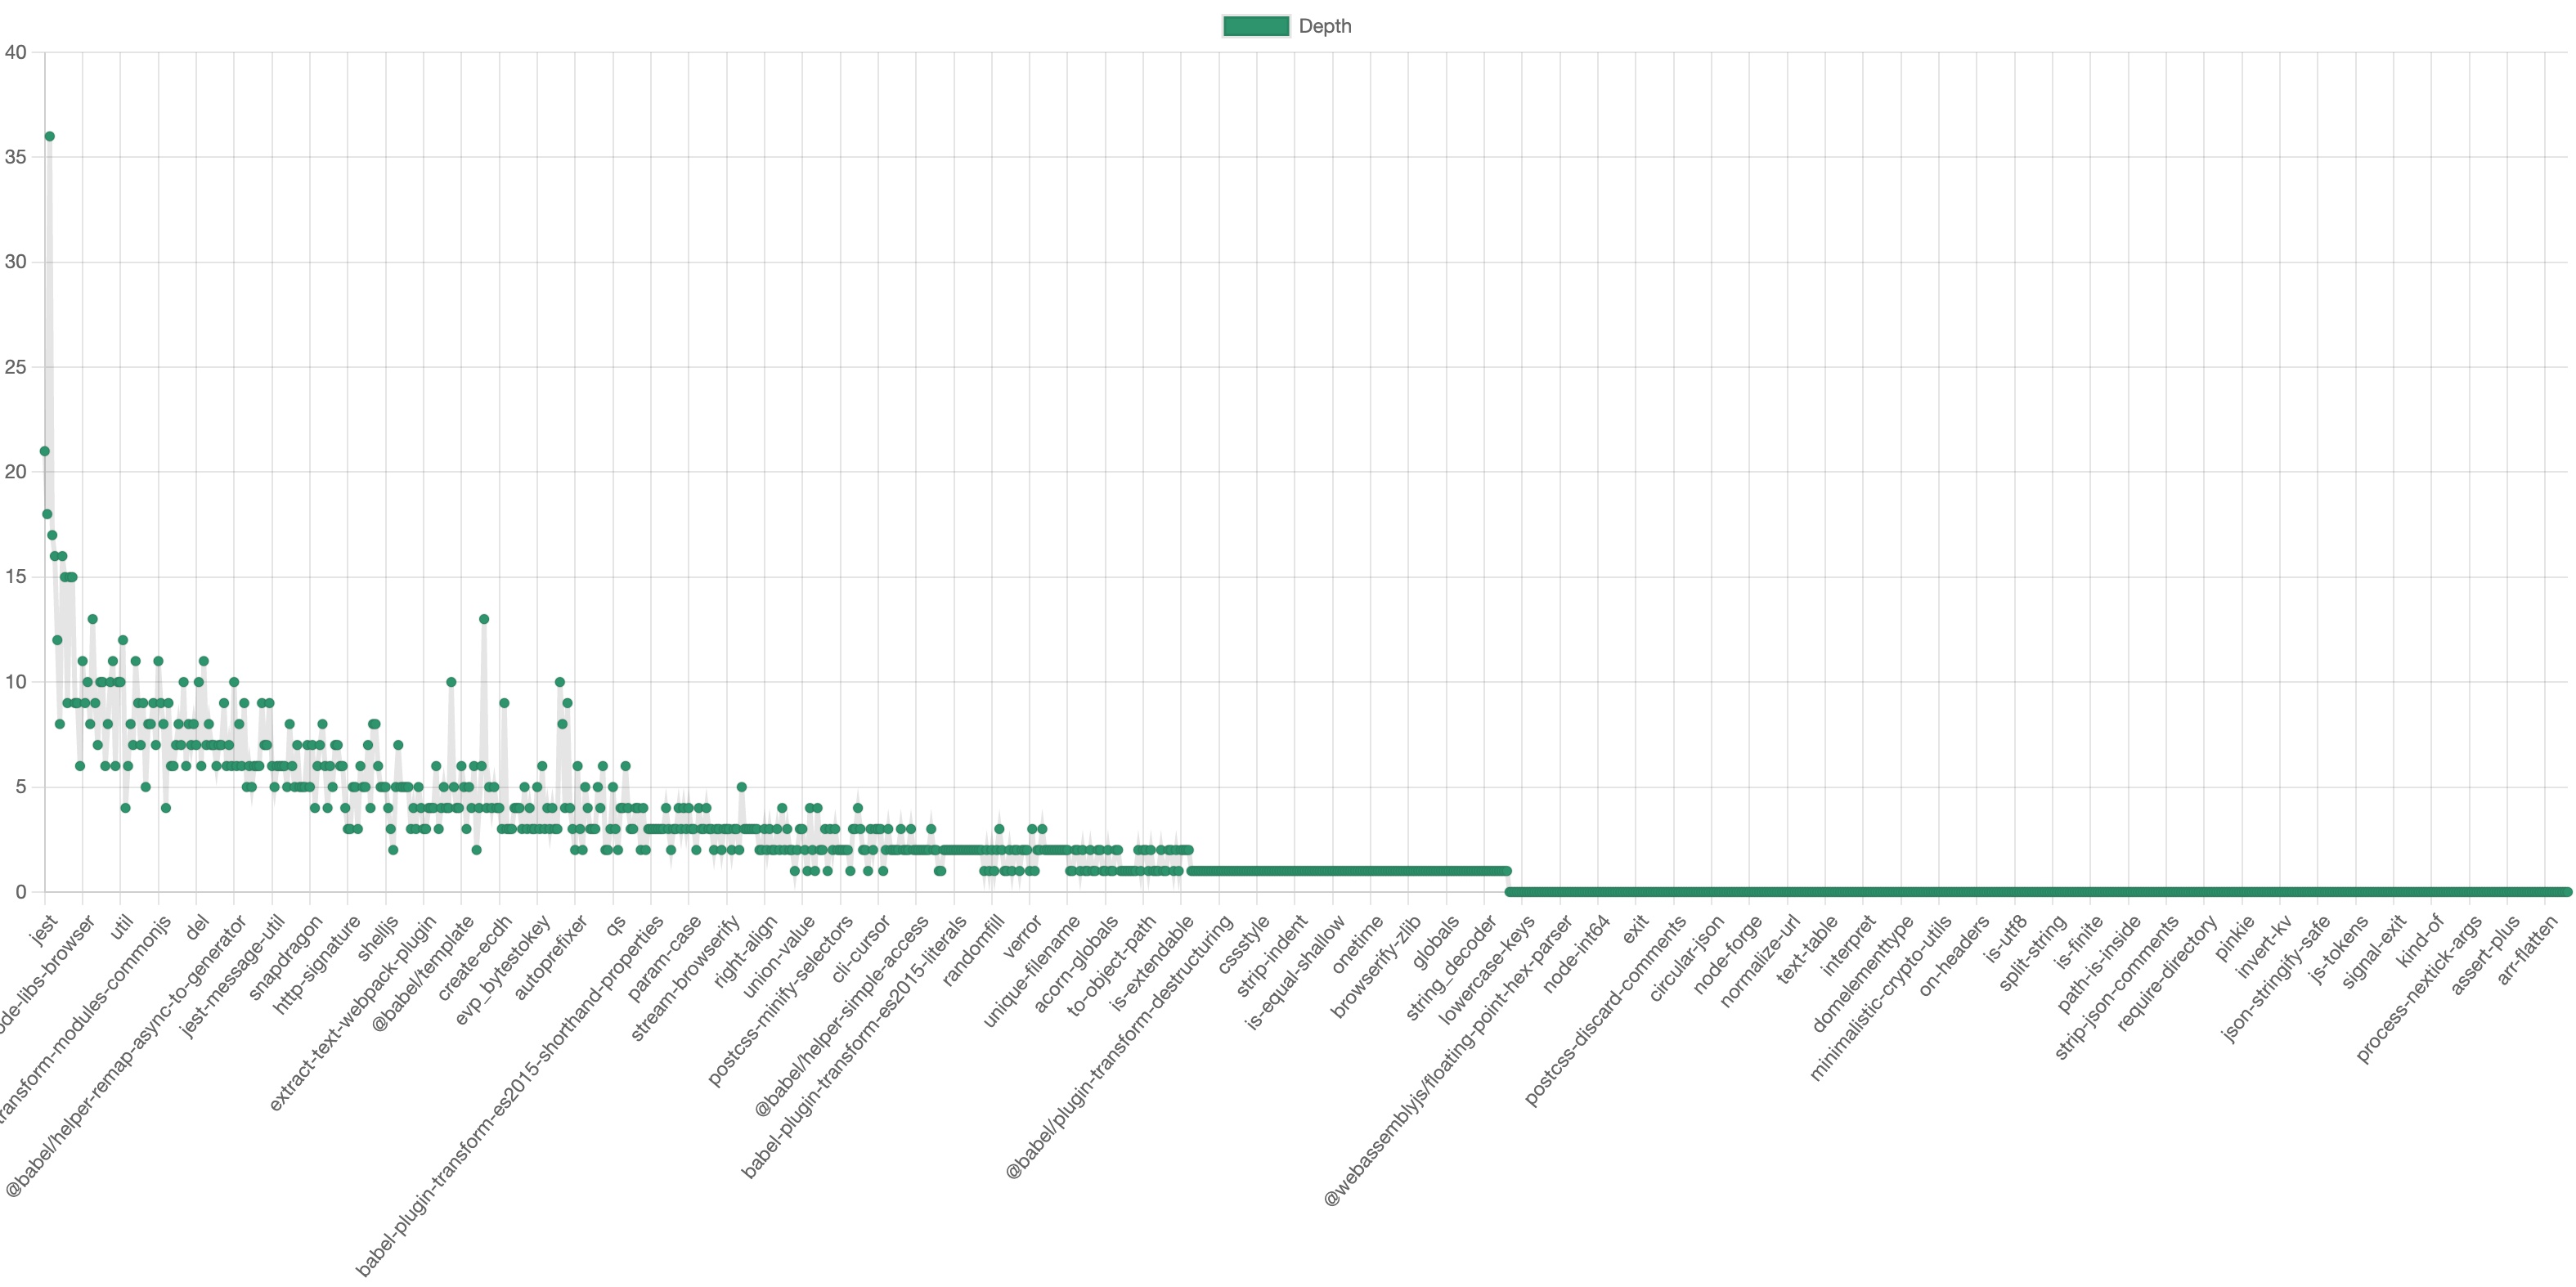
\includegraphics[scale=0.12]{images/graphdepth.png}
	\caption{Csomagonkénti gráfmélység}
	\label{fig:graphdepth}
\end{figure}

\begin{figure}[!h]
	\centering
	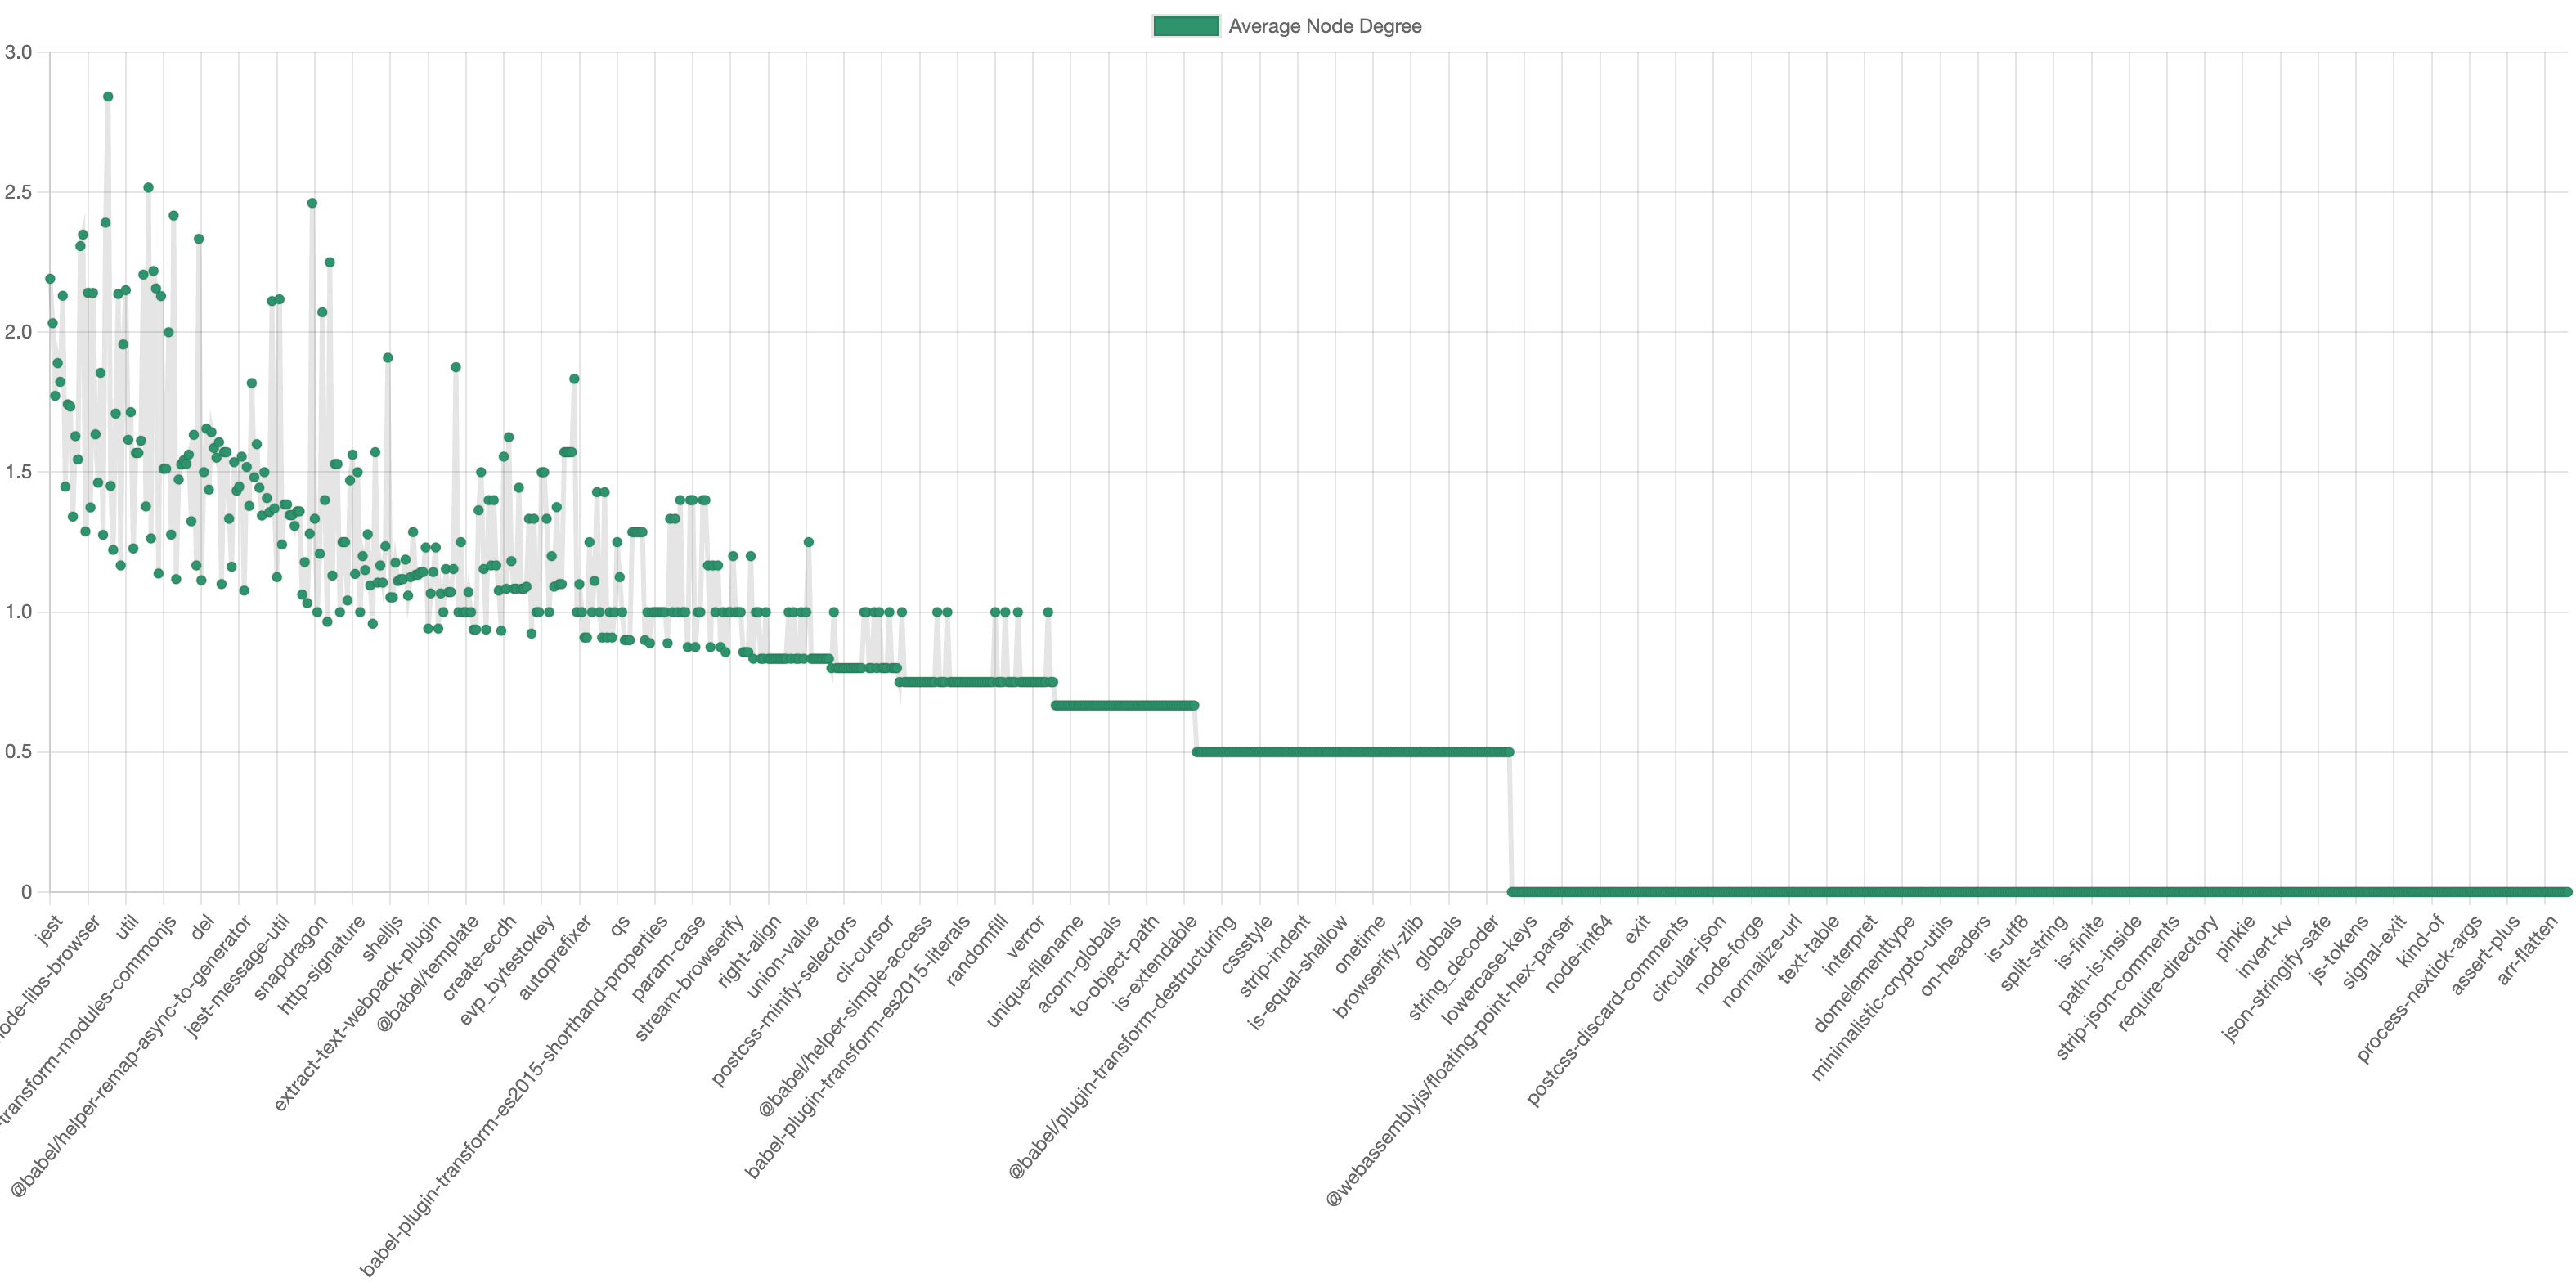
\includegraphics[scale=0.12]{images/avgdegree.png}
	\caption{Csomagonkénti átlagos fokszám}
	\label{fig:avgdegree}
\end{figure}

\begin{figure}[!h]
	\centering
	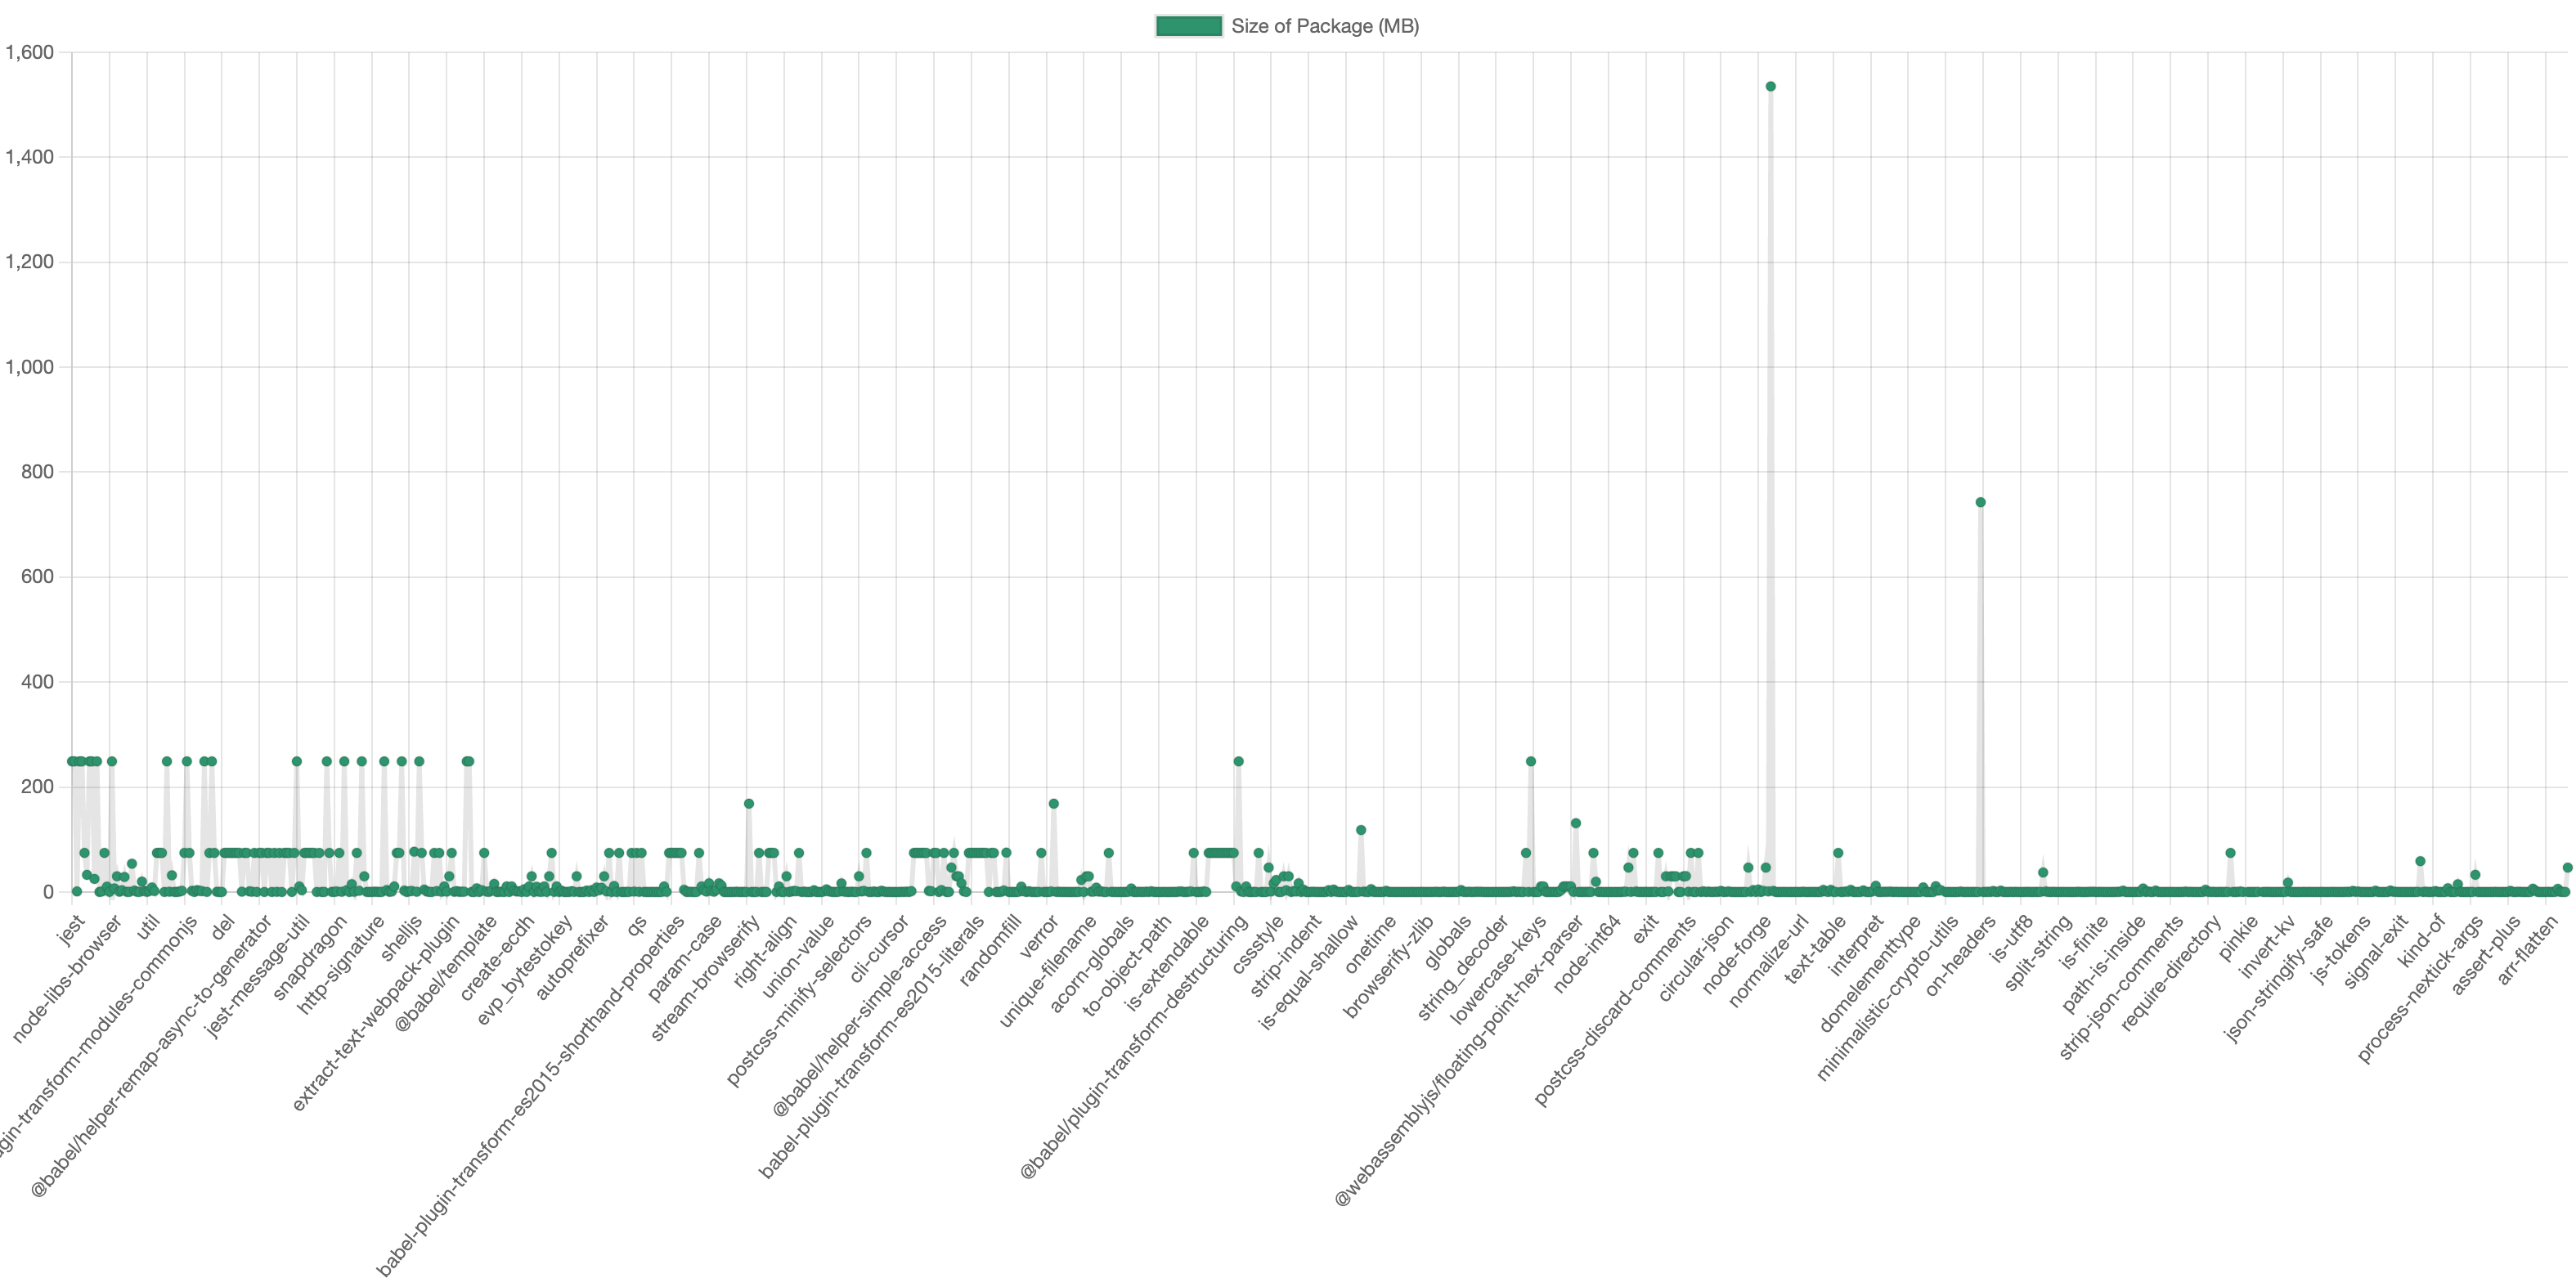
\includegraphics[scale=0.12]{images/pkgsize.png}
	\caption{Csomagok mérete(MB-ban megadott)}
	\label{fig:pkgsize}
\end{figure}

\begin{figure}[!h]
	\centering
	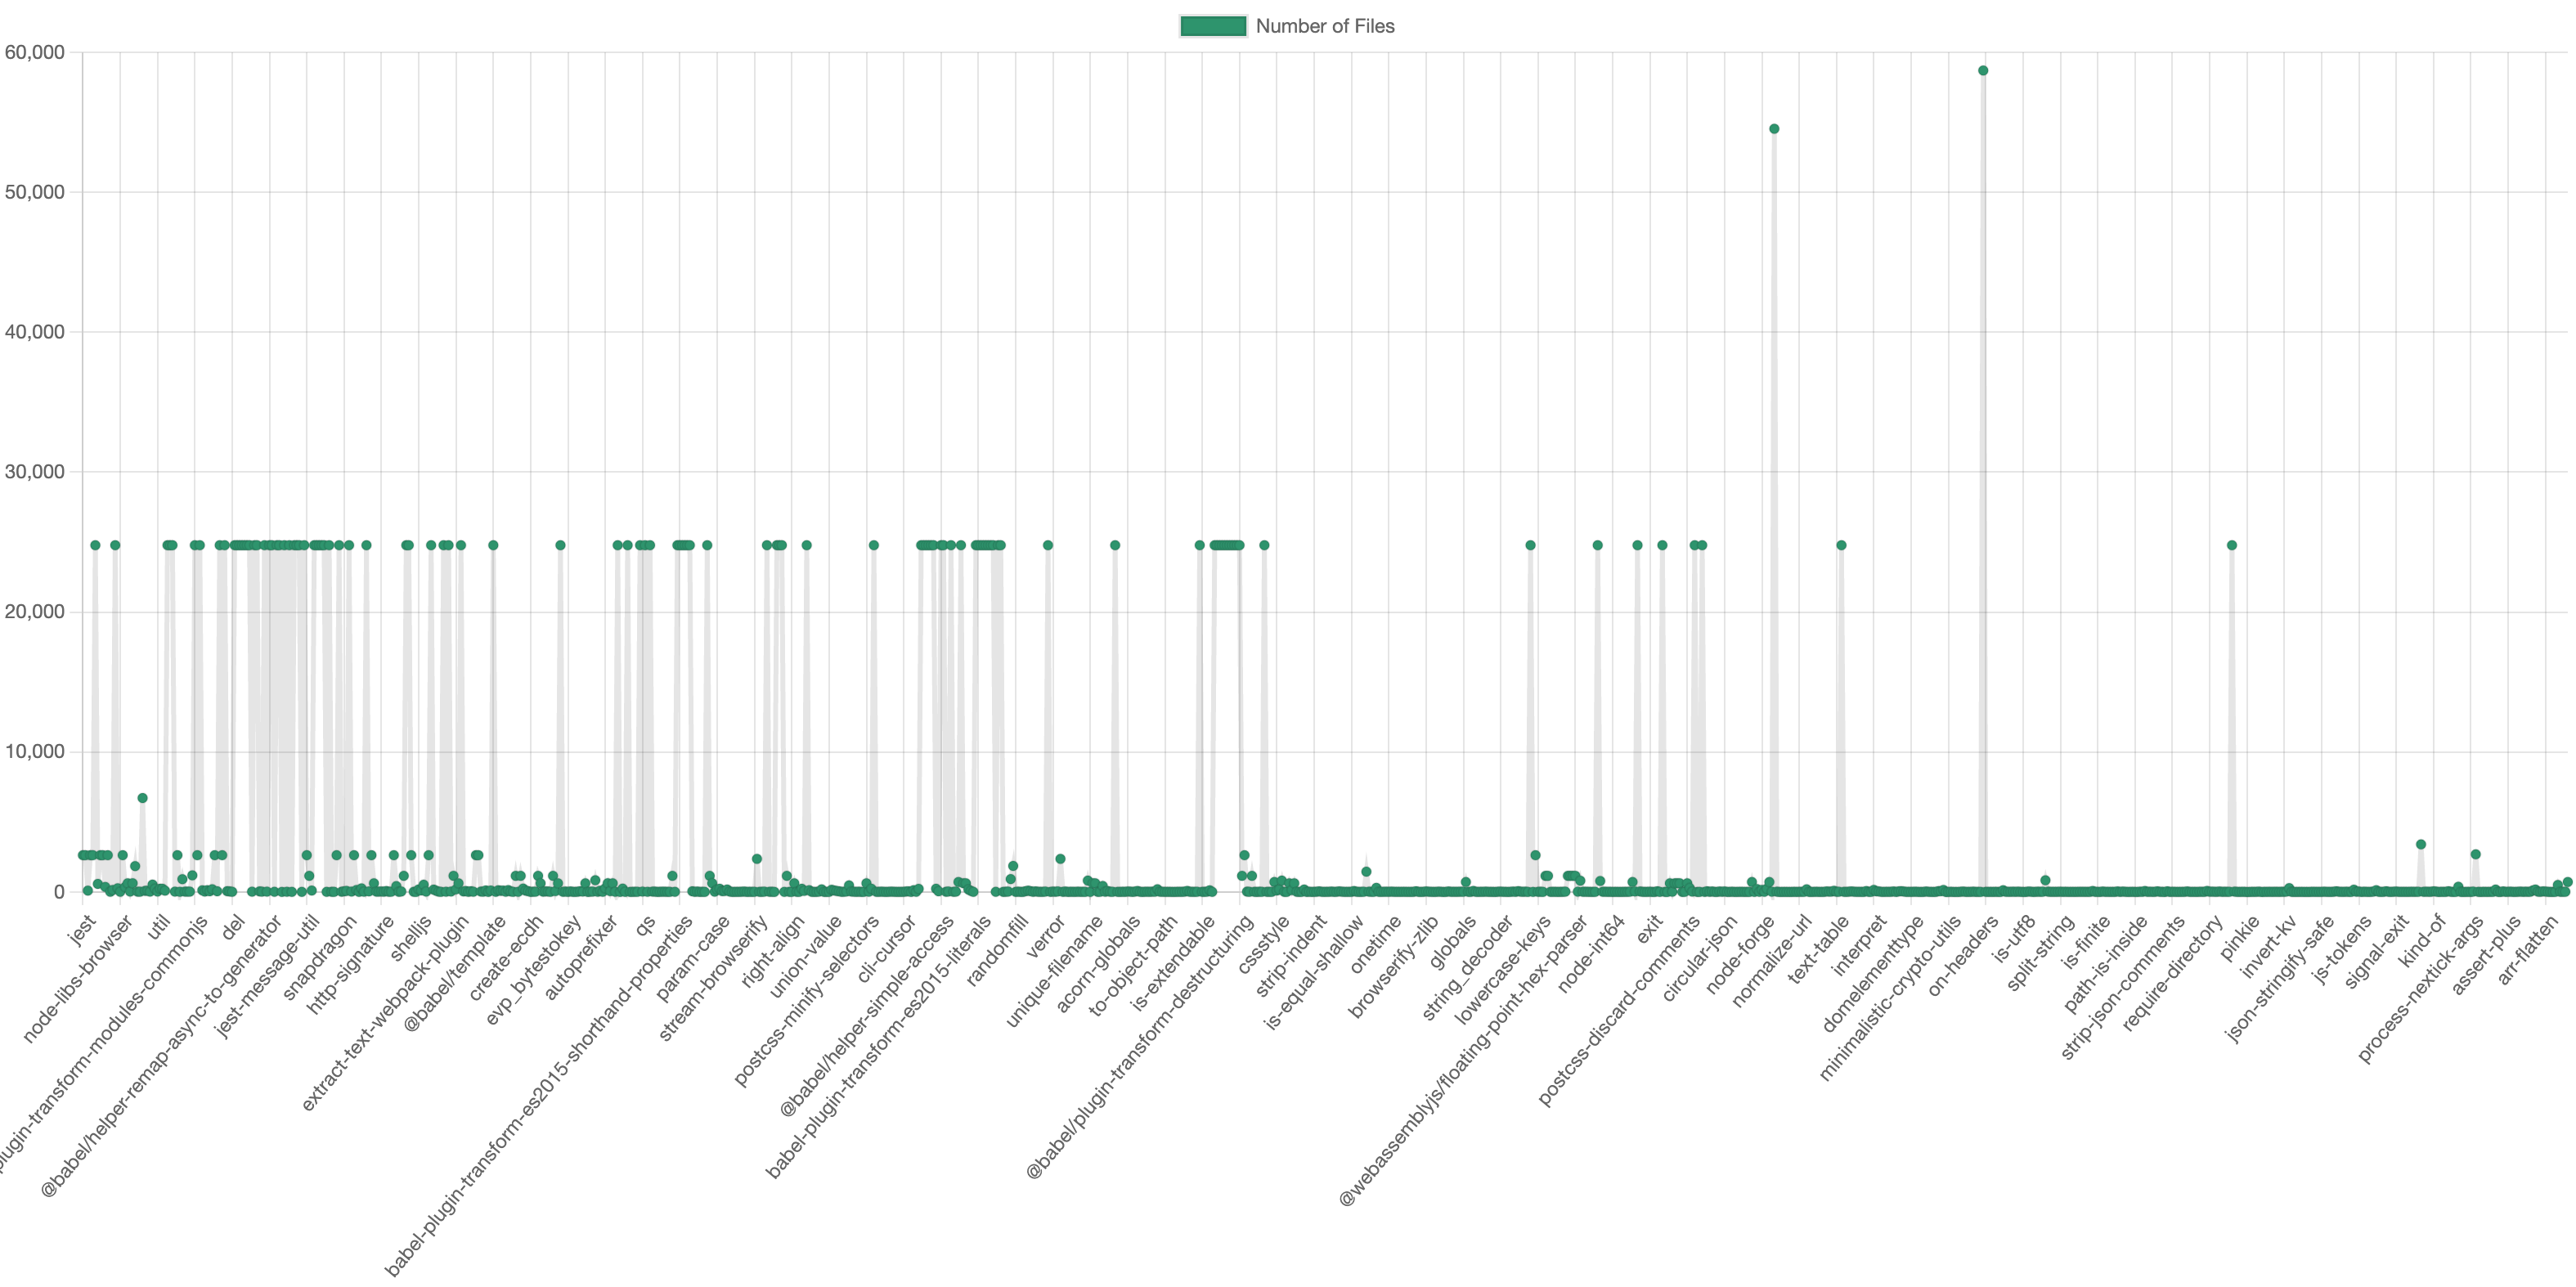
\includegraphics[scale=0.12]{images/numoffiles.png}
	\caption{Csomagonkénti fájlok száma}
	\label{fig:numoffiles}
\end{figure}

\begin{figure}[!h]
	\centering
	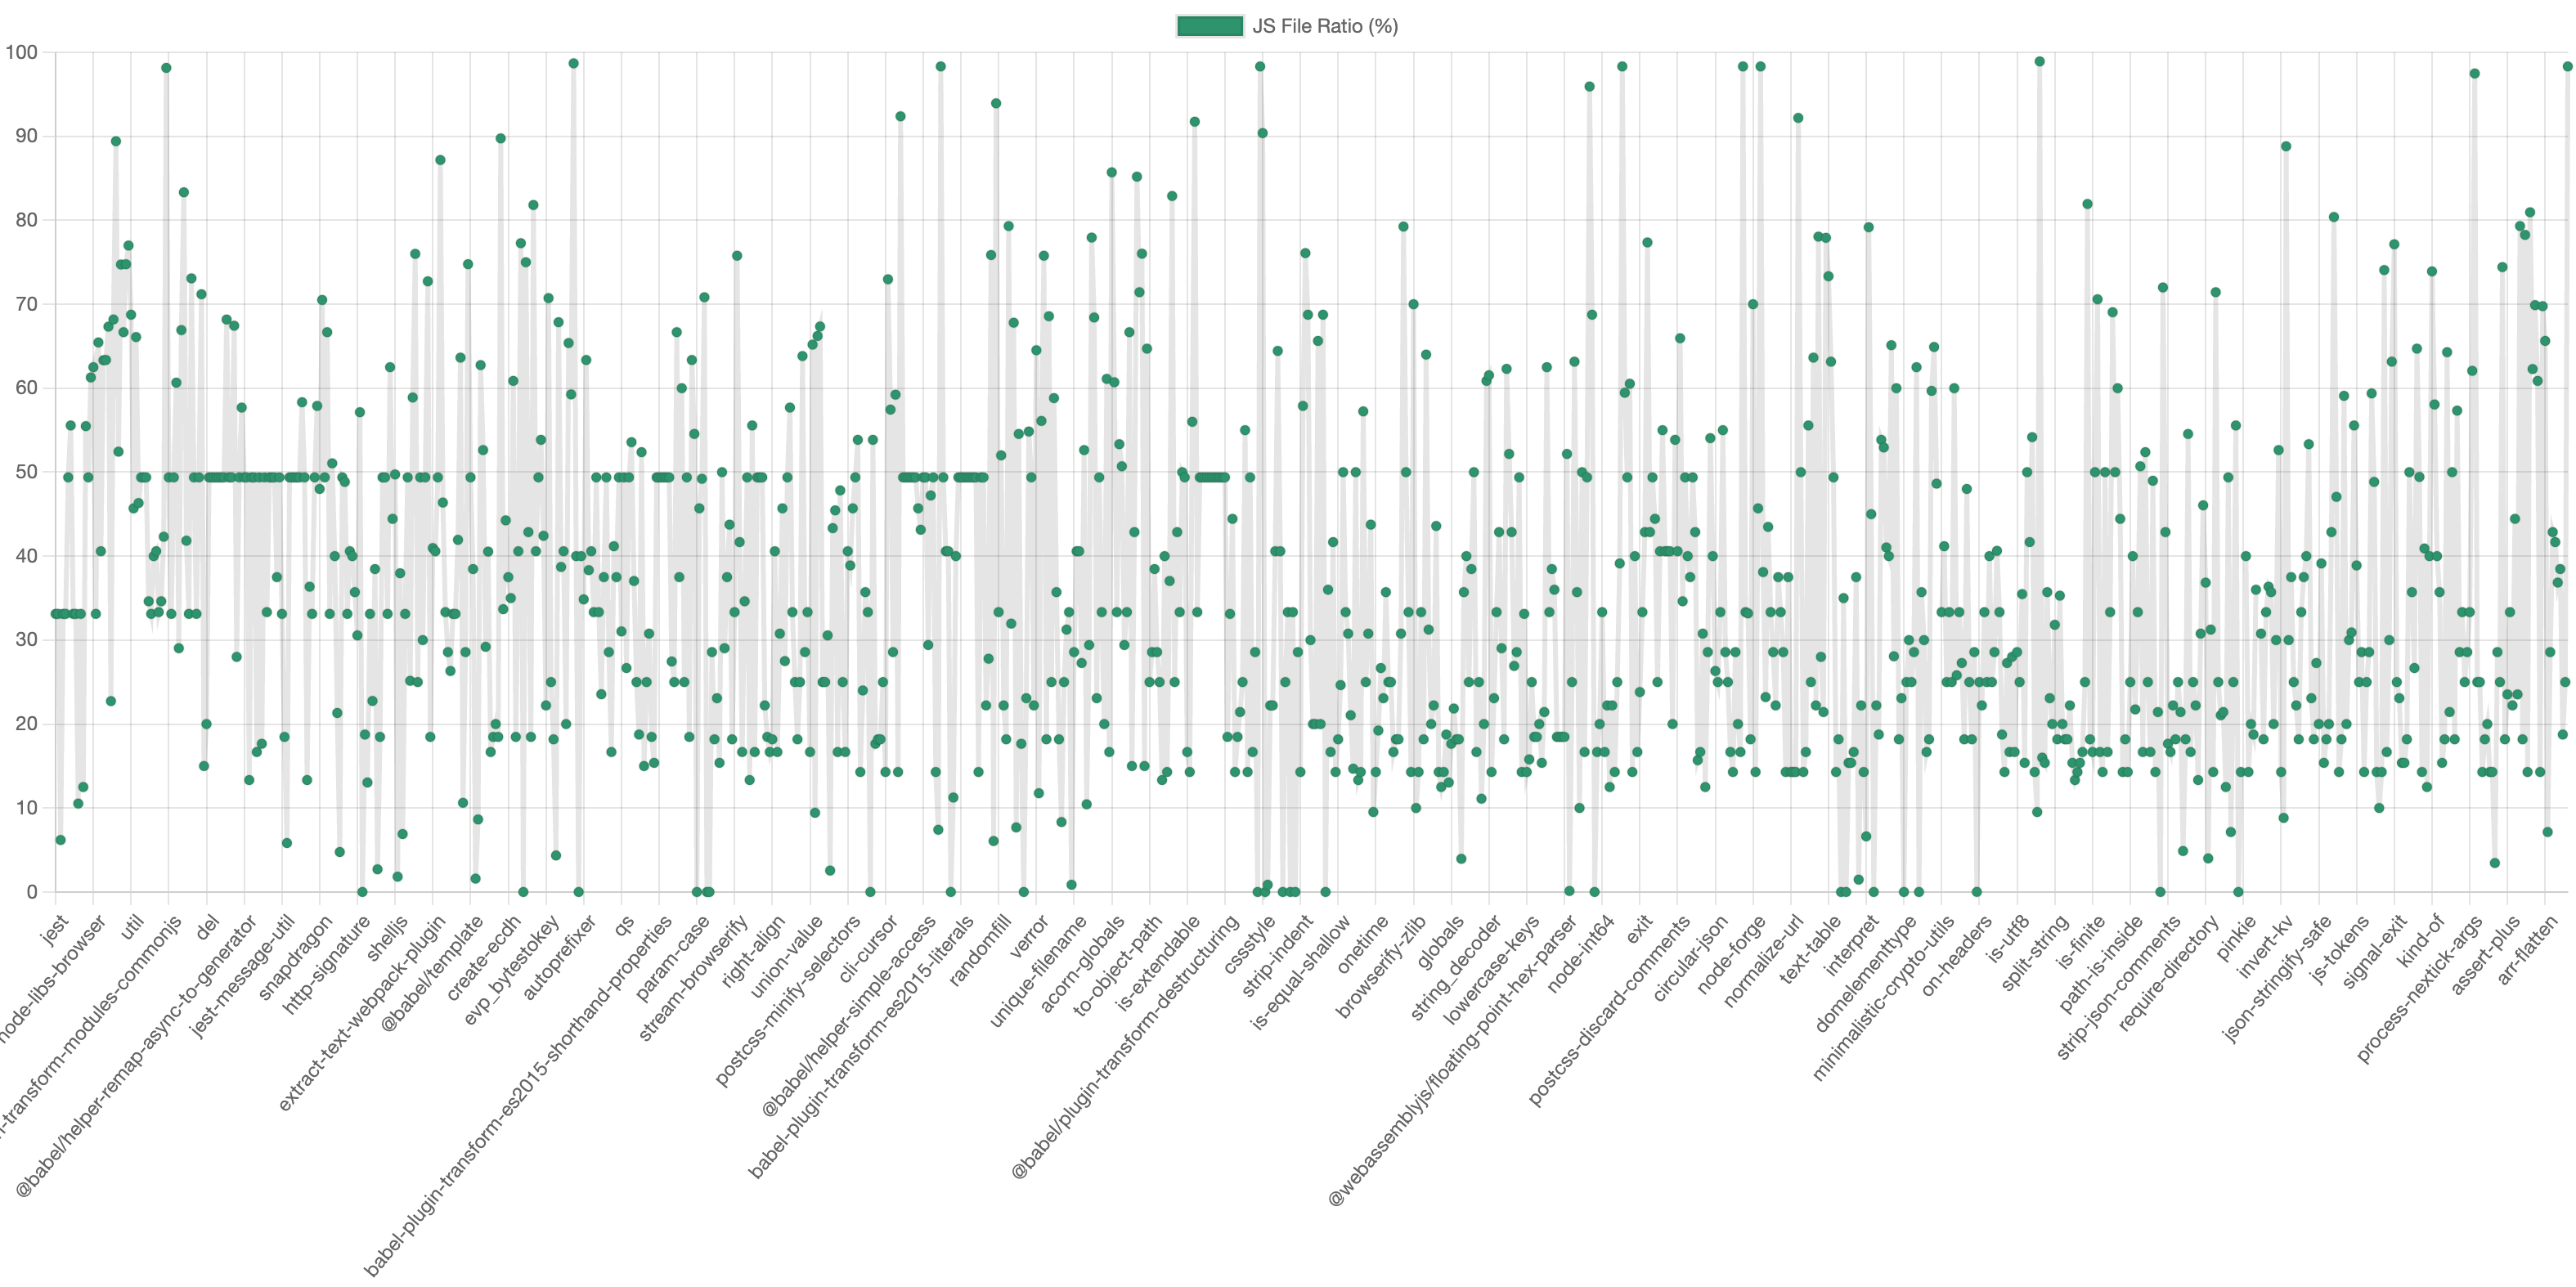
\includegraphics[scale=0.12]{images/jsratio.png}
	\caption{Csomagonkénti JavaScript fájlok aránya (\%)}
	\label{fig:jsratio}
\end{figure}

\begin{figure}[!h]
	\centering
	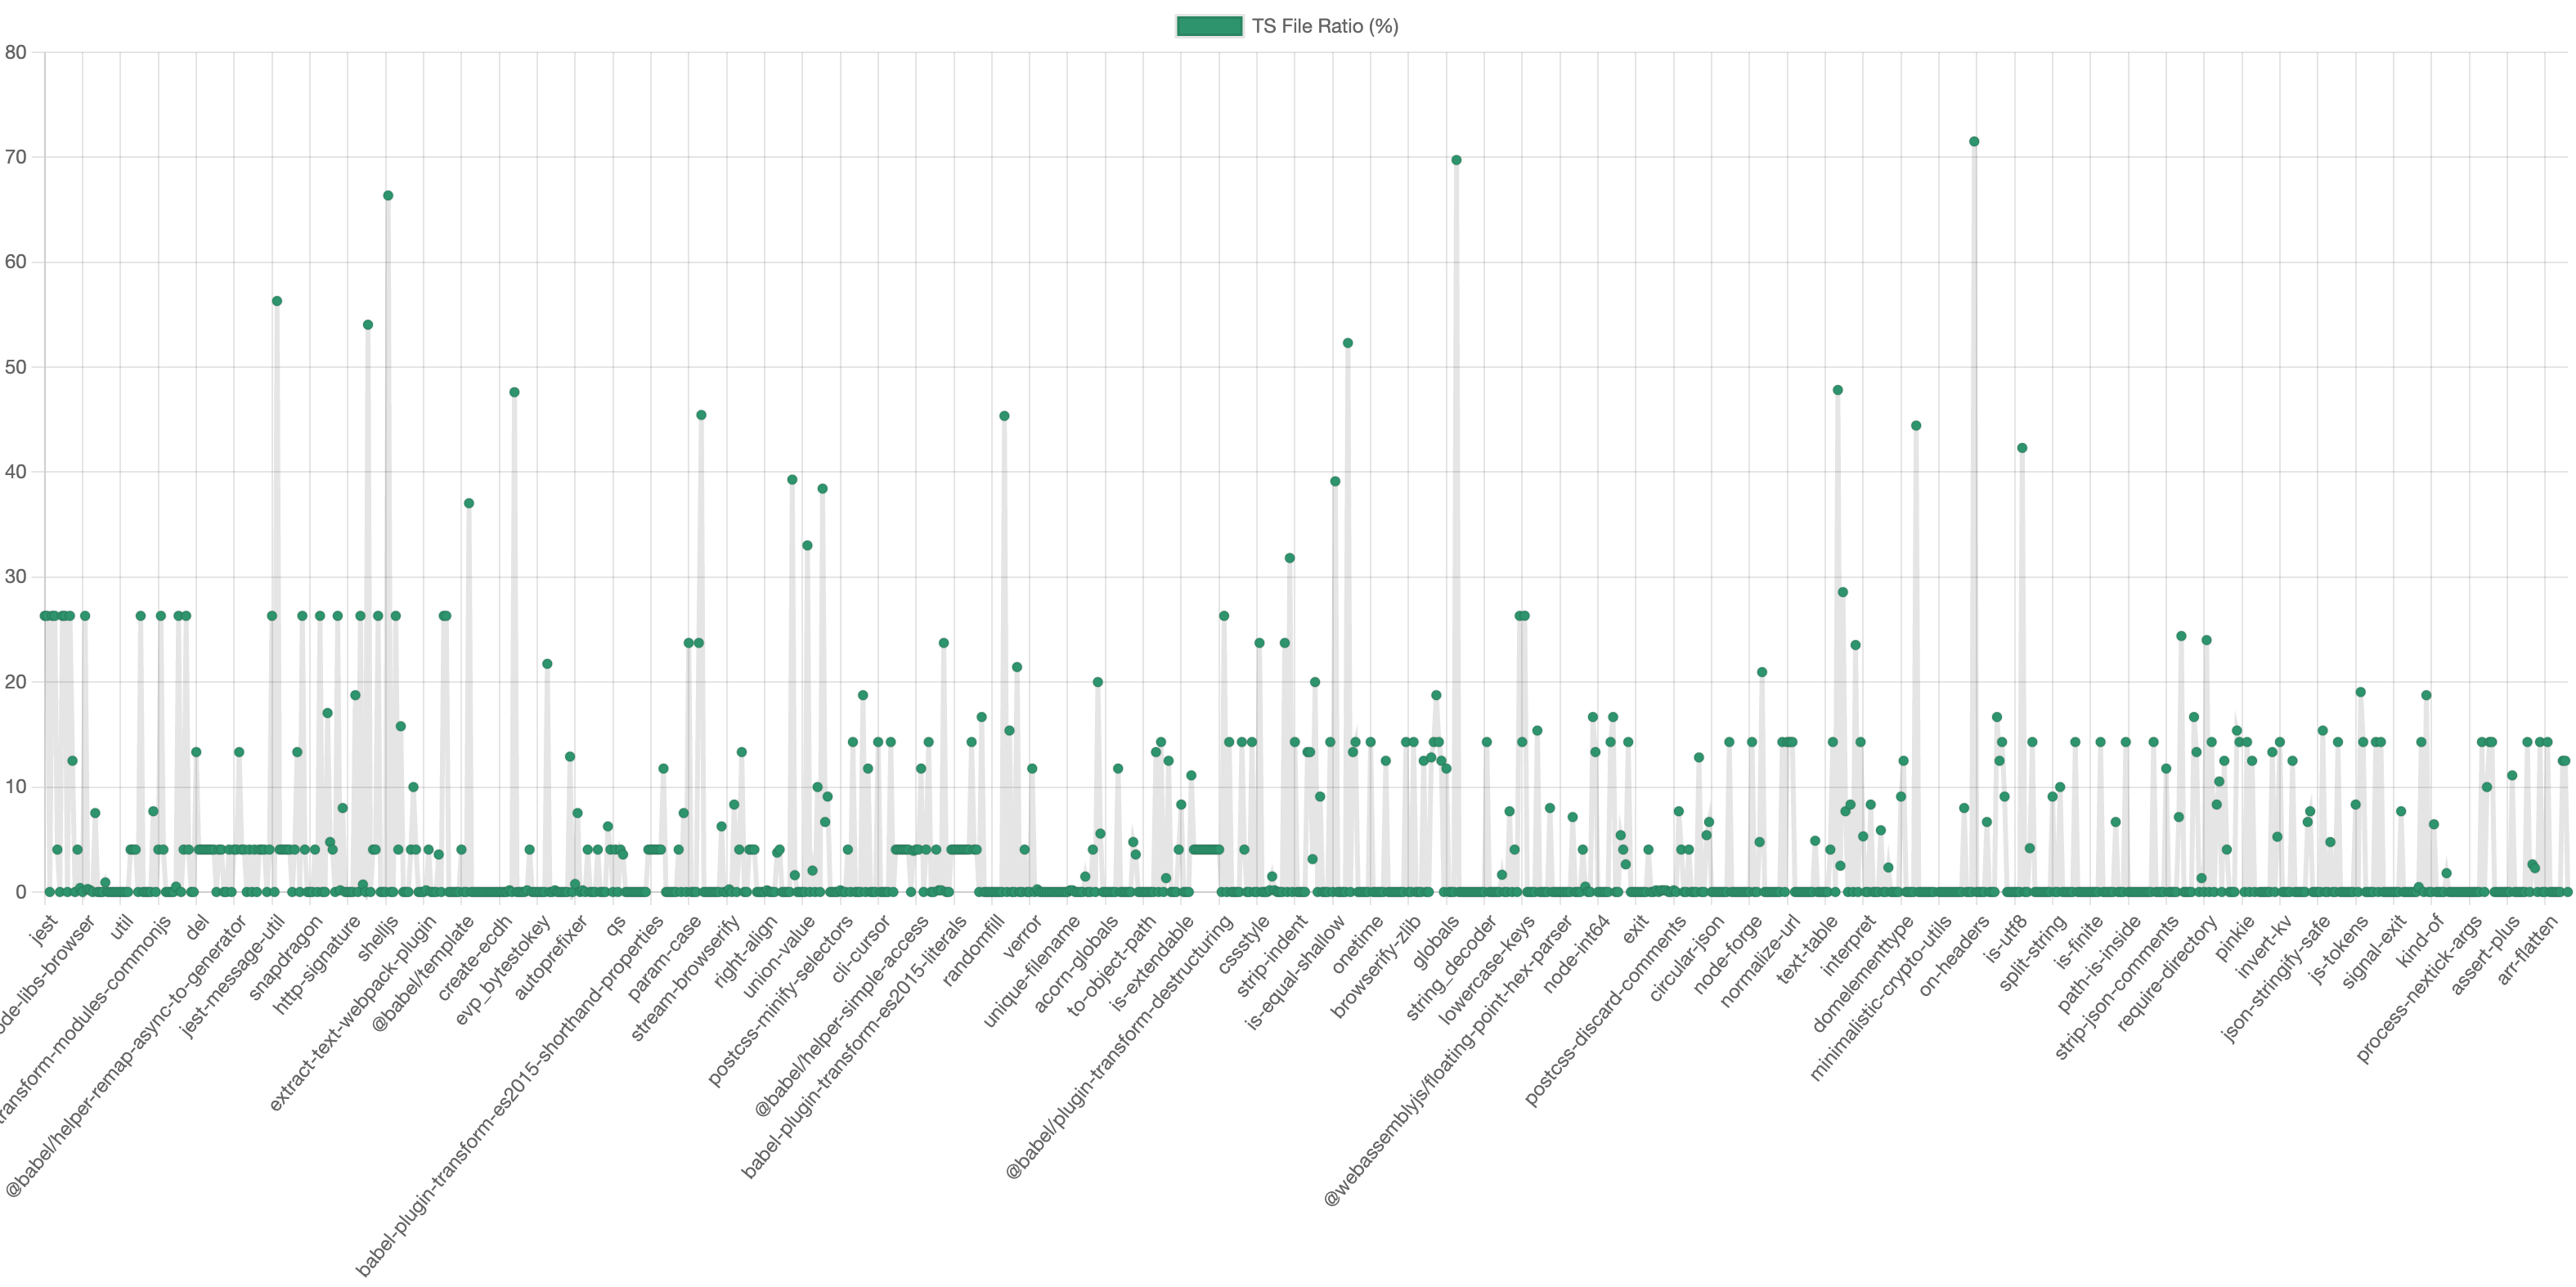
\includegraphics[scale=0.12]{images/tsratio.png}
	\caption{Csomagonkénti TypeScript fájlok aránya (\%)}
	\label{fig:tsratio}
\end{figure}

\pagebreak

\subsubsection{Eredmények Elemzése}

A program a számított hisztogramokat maga is elemezte, minden ábra esetében kiszámolta a prezentált adatok átlagát és szórását, melyet a Sidebar-ra írt ki az alábbi módon (Average = Átlag, Standard Deviation = Szórás)(\ref{fig:hg_data} ábra).

\begin{figure}[!h]
	\centering
	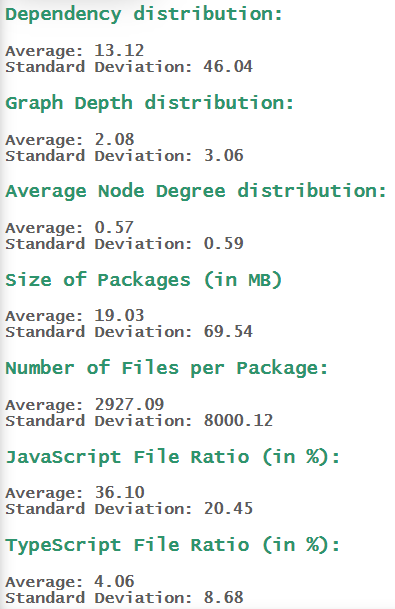
\includegraphics[scale=0.35]{images/hg_data.png}
	\caption{Eredmények elemzése}
	\label{fig:hg_data}
\end{figure}

A vizsgálat során minden csomag esetében a legutóbbi stabil verziót vette alapul a program. 

Az számítások és ábrázolás előtt a program a csomagokat a függőségek száma szerinti csökkenő sorrendbe rendezte, hogy egyértelműbbek legyenek az esetleges összefüggések.

\begin{itemize}
	\item Természetesen a gráf mélysége és a csomagok átlagos fokszáma, bár nem szigorúan, de követte a függőségek számának változását.
	\item A csomagméret esetében már ez a tendencia nem jelenik meg, bár alapvetően a nagyobb mennyiségű függőség esetében gyakoribb a nagy csomagméret.
	\item A csomagokban található fájlok mennyisége változó, de részben indikálja a csomag méretét.
	\item A JavaScript és TypeScript fájlok aránya az összes fájlhoz képest erősen inkonzisztens. Alapvetően elmondható, hogy a JavaScript alapú csomagok jóval gyakoribbak, mint a TypeScript alapúak.
\end{itemize}

\subsubsection{Az adatok eloszlása}

A kapott ábrák közül nem mindegyikről olvasható le egyértelmű konklúzió, ezért gyakorisághisztogramok készültek, amelyek már sokkal átláthatóbbak.\\

A \ref{fig:hist_1} ábra a 100-nál kevesebb fájlból álló csomagokban lévő fájl darabszámokat mutatja. Jól látható, hogy 10 körüli darabszámból van a legtöbb. Az 1000 vizsgált csomagból több mint a negyede ezen leszűkített tartományba esik.

\pagebreak

\begin{figure}[!h]
	\centering
	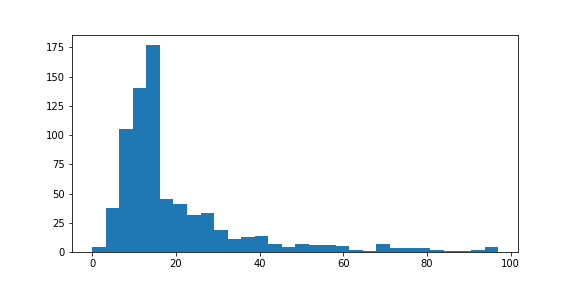
\includegraphics[scale=0.7]{images/hist_1.png}
	\caption{100-nál kevesebb fájlt tartalmazó csomagok}
	\label{fig:hist_1}
\end{figure}

A \ref{fig:hist_2} ábra már az 500 alatti darabszámokat jeleníti meg. A 100-as darabszám feletti tartományban alig fordulnak elő csomagok. 500 fájlszám felett hasonlóképpen elenyésző számban találni csak csomagokat.

\begin{figure}[!h]
	\centering
	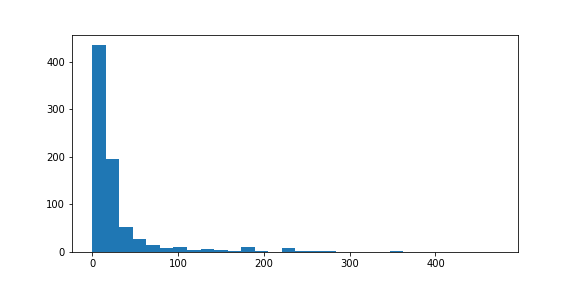
\includegraphics[scale=0.7]{images/hist_2.png}
	\caption{500-nál kevesebb fájlt tartalmazó csomagok}
	\label{fig:hist_2}
\end{figure}

A \ref{fig:hist_3} ábra a JavaScript fájlok arányának eloszlását jeleníti meg a csomagokban előforduló összes fájl számához viszonyítva. (A 0 azt jelzi, hogy egyáltalán nincs benne JavaScript fájl, az 1 pedig azt feltételezné, hogy csak azt tartalmaz, de a \emph{package.json} miatt ezt az értéket nem veheti fel.) A gyakorisághisztogram azt jelzi, hogy fájltípusok tekintetében a JavaScript fájlok egyáltalán nincsenek túlnyomó többségben a többi fájltípushoz képest. Érdekes eredmény, hogy 0,5 környékén egy kiugró érték van. Arról azt olvashatjuk le, hogy a vizsgált csomagok körülbelül nyolcadában a csomaghoz tartozó fájlok fele JavaScript állomány.

\begin{figure}[!h]
	\centering
	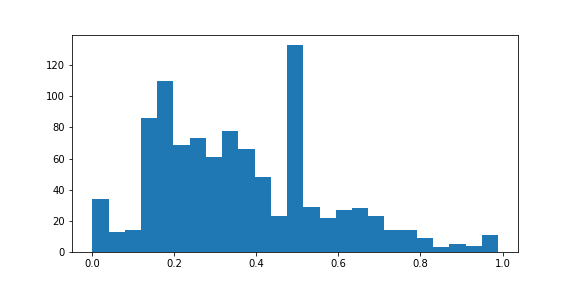
\includegraphics[scale=0.7]{images/hist_3.png}
	\caption{JavaScript fájlok arányának eloszlása}
	\label{fig:hist_3}
\end{figure}

\pagebreak

A \ref{fig:hist_4} ábra ugyanezen vizsgálatot a TypeScript fájlok esetére végzi. Az ábrából az állapítható meg, hogy a TypeScript fájlok a többi fájltípushoz képest igen kis arányban fordulnak elő.

\begin{figure}[!h]
	\centering
	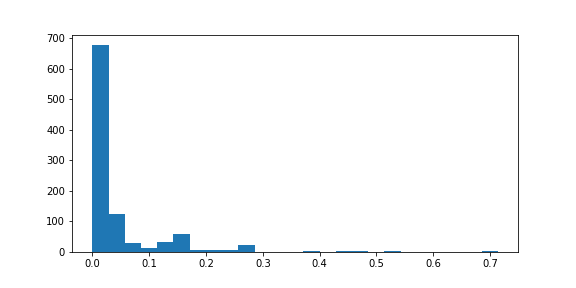
\includegraphics[scale=0.7]{images/hist_4.png}
	\caption{TypeScript fájlok arányának eloszlása}
	\label{fig:hist_4}
\end{figure}

\subsubsection{Érdekességek, kiugrások az ábrákon}

\begin{itemize}
	\item \textbf{Függőségek száma:} A legtöbb (400 feletti) függőséggel a \texttt{jest} (677), \texttt{jest}-\texttt{config} (569) és \texttt{gulp} (491) rendelkezik.
	\item \textbf{Gráf mélysége:} A \texttt{jest} 21 mélységű függőségi gráffal rendelkezik, amelyet indokol a függőségeinek száma, azonban a \texttt{gulp} érdekesebb, itt a kirívó 36-os mélység annak köszönhető, hogy található függőségi gráfjában nem várt kör, amely miatt az algoritmus tovább próbálta rendezni, sikertelenül a pontokat, míg végül feladta.
	\item \textbf{Átlagos fokszám}:  A \texttt{crypto-browserify} a maga 2,842-es átlagával volt a legmagasabb, de kirívónak nem nevezhető.
	\item \textbf{Csomagméret:} Két feltűnően nagy méretű csomag a \texttt{typescript} (1541,57 MB) és a \texttt{@types/node} (746,19 MB) amik maguk a TypeScript csomag és a Type-Script által használt Node.JS típusdefiníciókat tartalmazó csomag.
	\item \textbf{Fájlok száma:} Természetesen a két legnagyobb csomag kirívó itt is: \texttt{typescript} (54554 fájl), \texttt{@types/node} (58643 fájl).
	\item \textbf{TypeScript arány:} A JavaScript fájlok aránya változó, nincs kifejezetten kirívó eset, viszont a TypeScript esetében a \texttt{@types/node} típusdefiníciók 71,45\%-a TS fájl, illetve az ajv-keyword 79,74\%-a.
	\item \texttt{jest} és \texttt{babel}: A jest és babel scope-pal rendelkező csomagok és alcsomagok mind ugyanarra a GitHub linkre mutatnak a \emph{package.json} fájlban, mivel ugyanazon repositoryban található minden alcsomag, így a fájlszintű elemzések esetében (csomagméret, fájlok száma, TS és JS arányok) ugyanazokat az értékeket hozzák. Ez magyarázza ezeknél az ábráknál a több azonosan magas pontot.
	
\end{itemize}


\Section{A saját elemzőprogram elemzése}

A szoftver Node.JS csomagként is működik, a publikus npm registry-ben kiadásra került. Ennek köszönhetően a program tudja a saját függőségeit elemezni, amelyre az alábbi eredményt adta:

\begin{itemize}
	\item A függőségként megjelölt és használt 3 csomag közül a szemantikus verziózásért felelős \texttt{semver} két további függőségi szintet eredményezett, amely nem lett volna egyértelmű pusztán a \emph{package.json} tartalma alapján.
	\item Az elemzés során nem talált kulcsszavakban rejlő redundáns funkcionalitásra jeleket.
\end{itemize}

\begin{figure}[!h]
	\centering
	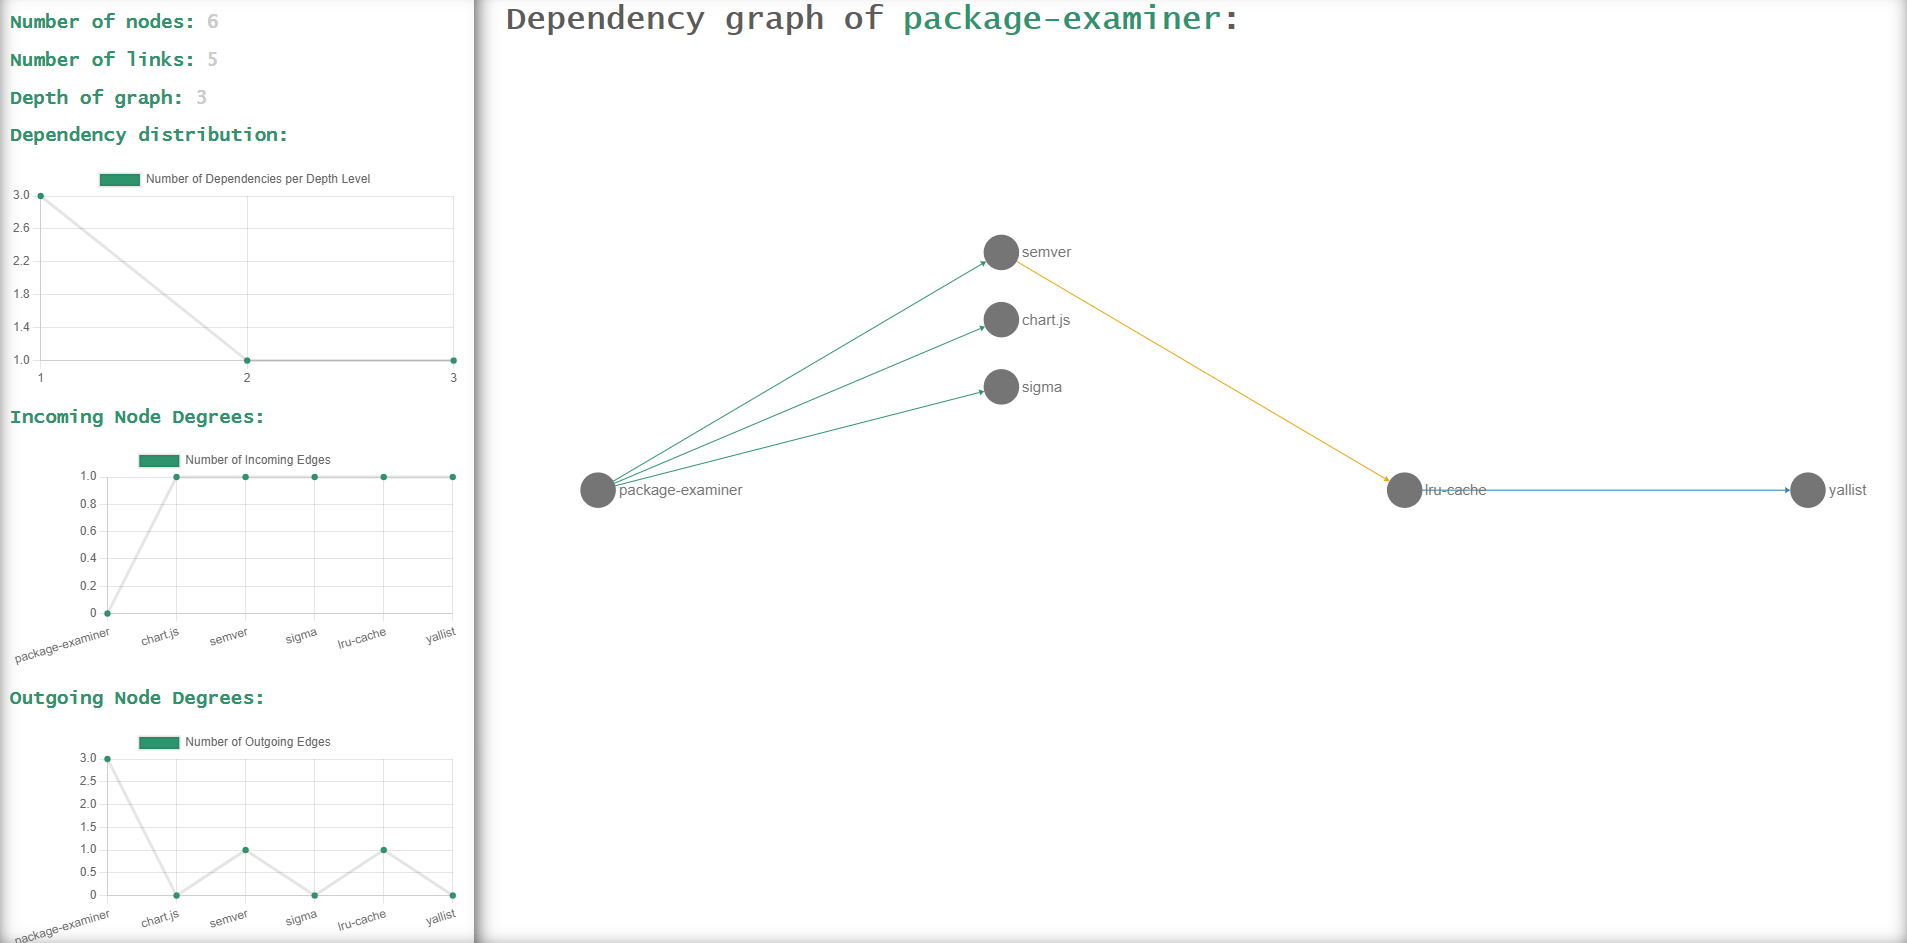
\includegraphics[scale=0.25]{images/package-examiner.png}
	\caption{A Package Examiner függőségeinek elemzése}
	\label{fig:package-examiner}
\end{figure}